%% Standalone source of one report figure. Rebuild: pdflatex -output-directory=.. fig-12-timeline.tex
\documentclass[11pt]{standalone}
\usepackage[T1]{fontenc}
\usepackage[utf8]{inputenc}
\usepackage{lmodern}
\usepackage{microtype}
\usepackage{amsmath,amssymb}
\usepackage{xcolor}
\usepackage{tikz}
\usetikzlibrary{arrows.meta,positioning,shapes.geometric,fit,calc,backgrounds}
\usepackage{pgfplots}
\usepackage{pgfplotstable}
\pgfplotsset{compat=1.18}
\setlength{\textwidth}{472.31595pt}  %% = the report's text width, so widths given in \textwidth match
\definecolor{gmblue}{HTML}{0B3D6E}
\definecolor{gmok}{HTML}{1E7B34}
\definecolor{gmwarn}{HTML}{B35C00}
\definecolor{gmbad}{HTML}{A32020}
\definecolor{gmgrey}{HTML}{5A5F66}
\definecolor{gmlight}{HTML}{EEF3F8}
\definecolor{gmteal}{HTML}{1B7A8C}
\newcommand{\done}{\textcolor{gmok}{\textbf{Done}}}
\newcommand{\partly}{\textcolor{gmwarn}{\textbf{Partly}}}
\newcommand{\pending}{\textcolor{gmbad}{\textbf{Pending}}}
\newcommand{\pass}{\textcolor{gmok}{\textbf{PASS}}}
\newcommand{\fail}{\textcolor{gmbad}{\textbf{FAIL}}}
\newcommand{\code}[1]{\texttt{\small #1}}
\newcommand{\INR}{INR~}
\newcommand{\gbar}[5]{\fill[#5] (#1,-#3+0.32) rectangle (#2,-#3-0.32);
  \node[anchor=east,font=\scriptsize] at (-0.3,-#3) {#4};}

\tikzset{
  box/.style={draw=gmblue, rounded corners=3pt, fill=gmlight, align=center, font=\small, inner sep=5pt,
              minimum height=9mm},
  gstep/.style={draw=gmblue, rounded corners=3pt, fill=white, align=center, font=\footnotesize, inner sep=4pt,
               text width=27mm, minimum height=11mm},
  st/.style={draw=gmblue, rounded corners=6pt, fill=gmlight, font=\scriptsize\ttfamily, inner sep=3pt,
             minimum height=6mm},
  arr/.style={-{Stealth[length=2.2mm]}, thick, gmblue},
  darr/.style={-{Stealth[length=2mm]}, gmgrey, dashed},
}

\begin{document}
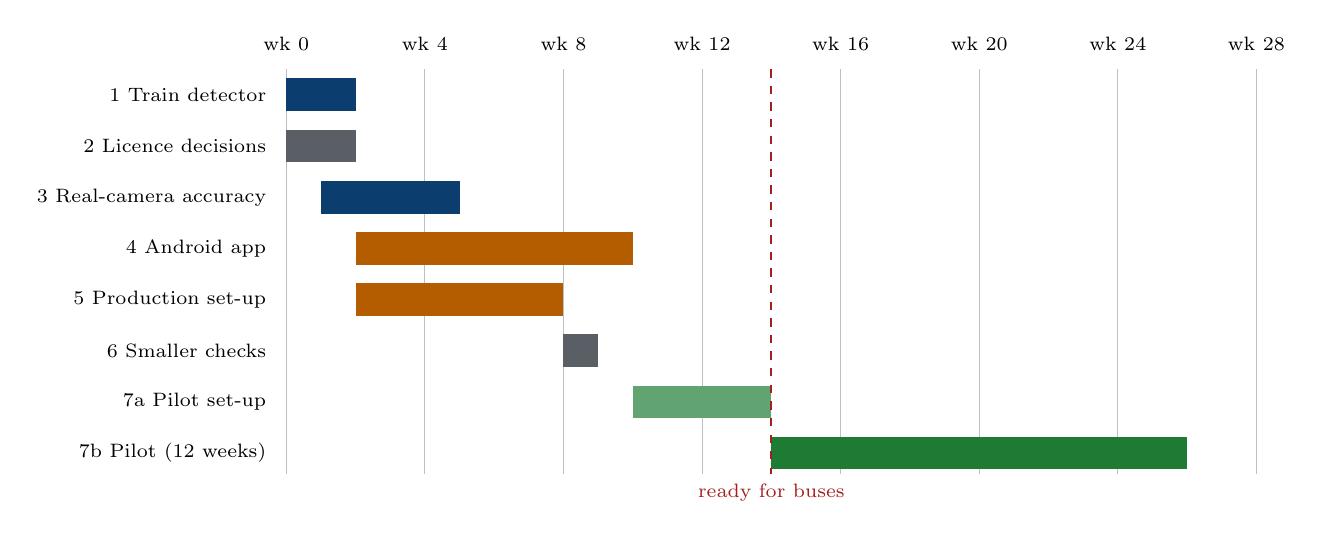
\begin{tikzpicture}[x=4.4mm, y=6.5mm]
  \foreach \w in {0,4,...,28}{ \draw[gmgrey!40] (\w,0.5)--(\w,-7.4); \node[font=\scriptsize] at (\w,1) {wk \w}; }
  \gbar{0}{2}{0}{1 Train detector}{gmblue}
  \gbar{0}{2}{1}{2 Licence decisions}{gmgrey}
  \gbar{1}{5}{2}{3 Real-camera accuracy}{gmblue}
  \gbar{2}{10}{3}{4 Android app}{gmwarn}
  \gbar{2}{8}{4}{5 Production set-up}{gmwarn}
  \gbar{8}{9}{5}{6 Smaller checks}{gmgrey}
  \gbar{10}{14}{6}{7a Pilot set-up}{gmok!70}
  \gbar{14}{26}{7}{7b Pilot (12 weeks)}{gmok}
  \draw[gmbad, thick, dashed] (14,0.5)--(14,-7.4) node[below, font=\scriptsize, text=gmbad] {ready for buses};
\end{tikzpicture}
\end{document}
